\documentclass[runningheads]{llncs}
\usepackage[T1]{fontenc}
\usepackage{amsmath,amssymb}
\usepackage{graphicx}
\usepackage{booktabs}
\usepackage{url}
\newcommand{\Cl}{\mathrm{Cl}}
\newcommand{\Z}{\mathbb{Z}}
\newcommand{\Q}{\mathbb{Q}}
\newcommand{\p}{\mathfrak{p}}

\begin{document}
\title{Regev's Factoring Algorithm over Class Groups:\\ Half the Group Operations,\\ More Than Twice the Cost}
\titlerunning{Regev's Factoring Algorithm over Class Groups}
\author{Anonymous Submission}
\authorrunning{Anonymous Submission}
\institute{}
\maketitle

\begin{abstract}
Regev's quantum factoring algorithm spends, summed over its runs, a number of sequential group operations proportional to the bit length of the group in which it collects relations. The class group of the imaginary quadratic field attached to the modulus has about half as many bits as the multiplicative group modulo the modulus, and its elements of order two are the factorization itself. We make the resulting algorithm explicit, with prime forms of small norm as the ``small elements'' that Eker\aa{} and G\"artner identified as the obstacle to generalizing Regev, prove the reduction from factoring to the class number, verify the classical post-processing on moduli up to 189 bits, and simulate the quantum sampler end to end, recovering the relation lattice exactly. We then cost the route at a 4096-bit modulus. Squaring a form contains a modular inverse with respect to a quantum modulus, and we argue this is intrinsic to the form model. Deriving the NUDUPL squaring identity, measuring its operation counts on real 4096-bit forms, and executing verified branch-free reversible designs for the inverse and the partial Euclidean reduction under one adder-cost convention, we find that a class-group squaring costs at least four times an integer squaring, five when fully uncomputed. After the halved operation count the route remains at least 2.4 times as expensive, 2.9 times when fully uncomputed, and its Euclidean components alone exceed the integer step by a factor of 2.3. We close with heuristic remarks on why a group of this size pays for its arithmetic.
\end{abstract}
\keywords{Integer factorization \and Quantum cryptanalysis \and Regev's algorithm \and Class groups \and Binary quadratic forms \and Quantum resource estimation}

\section{Introduction}
Shor factors $N$ by finding one long period in $(\Z/N\Z)^*$ \cite{shor1997}. Regev \cite{regev2023} replaces that with $d+4$ short runs, $d\approx\sqrt n$ for $n=\log_2N$, each computing a product $\prod g_i^{z_i}$ of $d$ small primes over a $d$-dimensional box of exponents, and recovers the lattice of multiplicative relations among the $g_i$ by lattice reduction. The gate cost per run drops from $\tilde O(n^2)$ to $\tilde O(n^{3/2})$; Ragavan and Vaikuntanathan \cite{ragavan2024} cut the space, Eker\aa{} and G\"artner \cite{ekera2024} added discrete logarithms, and Pilatte \cite{pilatte2024} proved the number-theoretic assumption for a variant of the algorithm. One accounting fact drives this paper: the total number of sequential squarings over all runs is about $\log_2|G|$ for the group $G$ supplying the relations, however the work is split between runs and precision.

Eker\aa{} and G\"artner observe that extending Regev to other groups needs a notion of small elements whose products stay small, and that this is not straightforward beyond $(\Z/N\Z)^*$. The class group $\Cl(-N)$ of binary quadratic forms of discriminant $-N$ has an obvious such notion: the prime forms $\p_\ell$ of small norm $\ell$, the factor base of Hafner and McCurley's classical algorithm \cite{hafner1989}. It has order $h\approx\sqrt N$, so $\log|G|$ is halved. And its order-two classes are ambiguous forms whose leading coefficients divide $N$, the mechanism of the 1984 Schnorr--Lenstra method \cite{schnorr1984}, so the factorization is read off the group structure with no probabilistic square-root step. Hallgren \cite{hallgren2005} computes class groups in quantum polynomial time, so a polynomial-time quantum factoring algorithm through this route has been implicit for twenty years; nobody wrote it down because Shor's algorithm already existed, and nobody costed it.

\textbf{This paper shows that Regev's algorithm over $\Cl(-N)$ performs half the sequential group operations of the integer version and still costs at least $2.4\times$ more ($2.9\times$ fully uncomputed), because squaring a form requires a modular inverse modulo quantum data that, we argue, no representation removes.} Fig.~\ref{fig:hero} is the result. Under identical adder costs at a 4096-bit modulus, one integer squaring step costs $17.0$ units, and the multiplications inside one class-group step, the NUDUPL products ($17.8$) together with those of the small-form composition ($8.2$), cost $26$ units before any Euclidean step is counted.

\paragraph{Contributions}
\begin{enumerate}
\item The algorithm, explicitly: generators, the quantum step, and the classical post-processing from recovered relation vectors to a factor, with a self-contained proof that factoring reduces to the class number (Sections~\ref{sec:prelim}--\ref{sec:alg}).
\item Verification: a classical implementation of the full pipeline factors five moduli from 59 to 189 bits, and a simulator of the quantum sampler in the style of Eker\aa's \texttt{regevnum} recovers the relation lattice with index one at 59 and 99 bits and factors (Section~\ref{sec:exp}); Lemma~\ref{lem:amb}, the uniqueness of reduced forms, the ambiguity of order-two reduced forms, and the group-theoretic part of Theorem~\ref{thm:red} are machine-checked in Lean~4; the class group itself enters only through its defining properties (Section~\ref{sec:repro}).
\item Cost: a derivation of the NUDUPL squaring identity with measured operation counts on real 4096-bit forms, a branch-free reversible modular inverse and a reversible partial Euclid both executed and verified, and a comparison under one convention (Section~\ref{sec:cost}).
\item Structure: why the inverse is intrinsic to the form model (Section~\ref{sec:cost}), and heuristic remarks on why a group of size about $\sqrt N$ pays for an inverse (Section~\ref{sec:disc}).
\end{enumerate}

\begin{figure}[t]
\centering
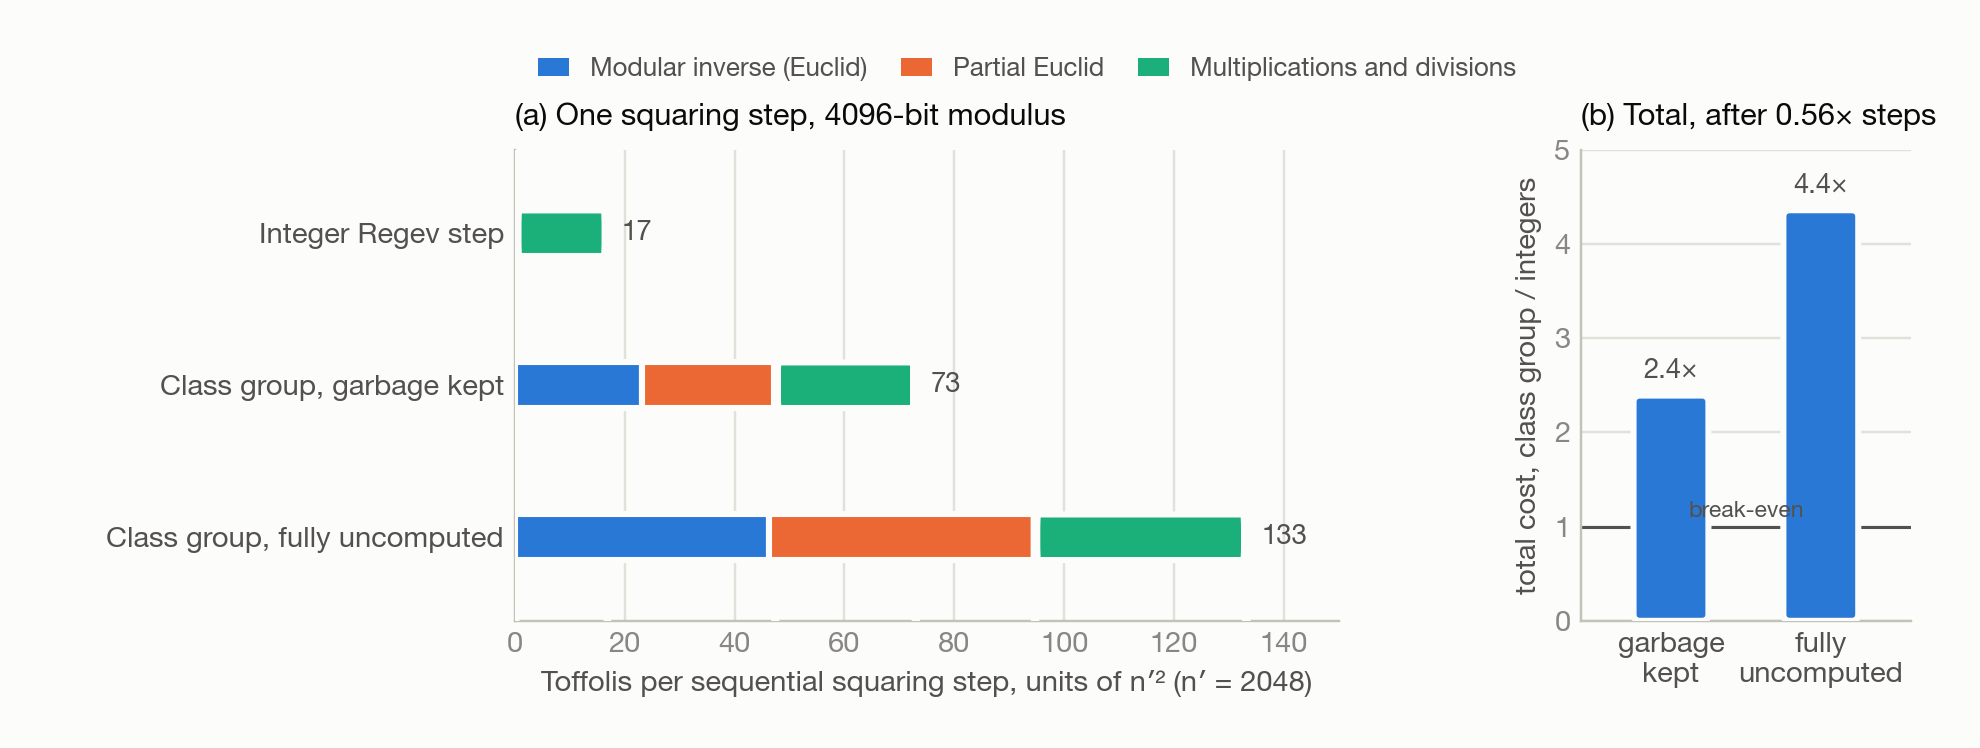
\includegraphics[width=0.96\textwidth]{fig_hero.png}
\caption{The verdict. (a) Toffoli cost of one sequential squaring step at a 4096-bit modulus, same adder costs for both routes, in units of $(n')^2$ with $n'=2048$. The integer step is a single modular squaring plus a small multiplication; its fully uncomputed variant applies the same $1.5\times$ arithmetic overhead as the class group. The class-group step is split into the modular inverse, the partial Euclidean reduction, and ordinary multiplications and divisions; the last of these alone exceeds the integer step. (b) Total cost ratio after crediting the class group with $0.56\times$ as many sequential steps; both variants remain above break-even.}
\label{fig:hero}
\end{figure}

\section{Related Work}
\paragraph{Classical factoring through class groups} Schnorr and Lenstra \cite{schnorr1984} raise a random form to a product of small prime powers and square down to an ambiguous form; Seysen and A.~K.~Lenstra turned this into relation collection, and Lenstra and Pomerance \cite{lenstra1992} proved $L[1/2,1+o(1)]$ using multipliers in place of GRH. Schoof \cite{schoof1982} pins the class number by baby-step giant-step after an analytic estimate in $\tilde O(N^{1/5})$ under GRH. We reuse the extraction mechanism unchanged and claim nothing classical.

\paragraph{Quantum computation of class groups} Hallgren \cite{hallgren2005} for constant degree and Biasse and Song \cite{biasse2016} for arbitrary degree compute class groups in quantum polynomial time, which with the standard reduction \cite{cohen1993} implies quantum factoring as a corollary. Schmidt gave a qubit estimate for class-group discrete logarithms \cite{schmidt2006} and the half-size representation by reduced forms \cite{schmidt2009}. These results supply the algorithm's existence; we supply its explicit Regev form and its cost.

\paragraph{The Regev family} Beyond \cite{regev2023,ragavan2024,ekera2024,pilatte2024}, Luo, Li and Le Gall \cite{luo2026} generalize the lattice post-processing to arbitrary abelian black-box groups, at a cost of $\tilde O(n^{3/2})$ group operations of cost $T_{\mathrm{op}}$ each, without naming a group. We instantiate the group they leave abstract and measure $T_{\mathrm{op}}$.

\paragraph{Quantum arithmetic} Roetteler et al.~\cite{roetteler2017} and Luo et al.~\cite{luo2026b} give reversible modular inverses at $4.2\times$ and $13.5\times$ their respective multipliers; Bernstein and Yang \cite{bernstein2019} give the constant-time divstep we build on; David, Espitau and Hosoyamada \cite{david2022} built a quantum circuit for reducing forms but not for composing them; Jacobson and van der Poorten \cite{jacobson2002} analyze NUCOMP classically. Gidney \cite{gidney2025}, on Chevignard et al.~\cite{chevignard2024}, gives the best Shor-type estimate, but its windowed classical-constant multiplications and residue arithmetic are unavailable to any circuit that squares a quantum register, so our comparison is within the Regev family.

\paragraph{Positioning} The four families meet at one question none of them asks: what does a Regev-style run cost in a group whose order is $\sqrt N$ rather than $N$? The classical literature supplies the extraction mechanism, the quantum class-group literature supplies existence, the Regev literature supplies the accounting that makes the group size matter, and the circuit literature supplies the primitives, with inverse-to-multiplication ratios reported against baselines too different to combine. Nobody had measured the composition cost of forms against a modular squaring under one convention, and the two published ratios bracket the break-even point so widely that the answer could not be inferred. This paper combines the four.

\section{Preliminaries and the Reduction}\label{sec:prelim}
\subsection{Forms}
A primitive positive definite form $(a,b,c)$ of discriminant $D=b^2-4ac<0$ is \emph{reduced} if $|b|\le a\le c$, with $b\ge0$ when $|b|=a$ or $a=c$; each class has exactly one reduced form, and $a\le\sqrt{|D|/3}$. Composition makes the classes a finite abelian group $\Cl(D)$ with $h(D)=\sqrt{|D|}L(1,\chi_D)/\pi$ elements. We take $N=pq$, $N\equiv3\pmod4$, $D=-N$, so $D$ is fundamental, the identity is $(1,1,(1+N)/4)$ and $b$ is always odd. For a prime $\ell$ with $(D/\ell)=1$ the prime form is $\p_\ell=(\ell,b_\ell,(b_\ell^2-D)/4\ell)$; under GRH the $\p_\ell$ with $\ell\le6\log^2|D|$ generate $\Cl(D)$ \cite{bach1990}.

\subsection{Regev's accounting}
For generators $g_1,\dots,g_d$ of an abelian group let $L=\{z:\prod g_i^{z_i}=1\}$, so $\det L=|\langle g_i\rangle|\le|G|$. A run prepares $\sum_z|z\rangle|\prod g_i^{z_i}\rangle$ over $z\in[0,2^B)^d$ by $B$ sequential squarings, measures the second register and Fourier-transforms the first, yielding a noisy point of $L^*/\Z^d$. After $m=d+4$ runs, LLL recovers a short basis of $L$ \cite{regev2023}, provided $2^B$ exceeds the short-basis length, heuristically $2^{\log_2|G|/d}\sqrt d$. The total number of sequential squarings is therefore
\begin{equation}\label{eq:total}
(d+4)\Big(\frac{\log_2|G|}{d}+c\Big)=\log_2|G|\,(1+4/d)+c\,(d+4),
\end{equation}
where $c$ is the slack in exponent bits beyond the short-basis length (we use $c=8$). The total is proportional to $\log|G|$ and nearly independent of $d$; for $|G|\approx\sqrt N$ it is half of the integer value.

\subsection{Factoring from the class number}
\begin{lemma}\label{lem:amb}
For $D=-N$, $N=pq$, every reduced form of order dividing $2$ is ambiguous ($b=0$, $b=a$, or $a=c$), and every non-identity one yields a proper factor of $N$.
\end{lemma}
\begin{proof}
The first claim is classical \cite{cohen1993}. $b=0$ is impossible since $D$ is odd. If $b=a$, $D=a(a-4c)$, so $a\mid N$ with $1<a\le\sqrt{N/3}<N$ unless $a=1$, the identity. If $a=c$, $-N=(b-2a)(b+2a)$ with $0\le b\le a$, so $0<2a-b<N$ divides $N$ and is proper unless $2a-b=1$, which forces $a=1$.
\end{proof}
\begin{theorem}\label{thm:red}
Given $h=|\Cl(-N)|$, $p$ and $q$ are found in expected polynomial time, using GRH only to sample a class of even order.
\end{theorem}
\begin{proof}
Genus theory gives $\Cl(D)[2]\cong(\Z/2)^{t-1}$ with $t=2$ primes dividing $D$, so the Sylow $2$-subgroup is cyclic of order $2^k$, $k\ge1$, and $h=2^km$ with $m$ odd. For a class $g$ with $g^m\ne1$, squaring $g^m$ at most $k-1$ times reaches the unique order-$2$ element, which factors $N$ by Lemma~\ref{lem:amb}. Classes with $g^m=1$ form a subgroup of index $2^k\ge2$, so at least half succeed; under GRH, random products of Bach's prime forms are nearly uniform, so a constant number of trials suffices.
\end{proof}
The converse is open: $p,q$ give no fast route to $h$. We ran the theorem with PARI \cite{pari} as the oracle for $h$ at 100 bits: one class, one exponentiation and five squarings produced a prime factor.

\paragraph{Moduli with $N\equiv1\pmod4$} Theorem~\ref{thm:red} and our experiments cover $N\equiv3\pmod4$. Otherwise $-N$ is not a discriminant and one takes $D=-4N$; then $t=3$, $\Cl(D)[2]\cong(\Z/2)^2$, and the descent of Theorem~\ref{thm:red} ends at one of three classes of order two. On all $207$ moduli $N\equiv1\pmod4$ below $2100$ that are products of two distinct primes, these are represented by $(2,2,(N+1)/2)$, which yields only the factor $2$, and by two ambiguous forms whose extracted value has a proper common factor with $N$. Which class the descent reaches depends on the structure of the Sylow $2$-subgroup, so the probability argument of Theorem~\ref{thm:red} does not carry over; Lenstra and Pomerance handle this case with multipliers \cite{lenstra1992}, and we do not analyse it further.

\section{The Algorithm}\label{sec:alg}
\paragraph{Generators} the $d$ smallest split primes; at $n=4096$, $d=64$ and $\ell_d$ lies between $587$ and $853$ on eight sampled moduli.

\paragraph{Quantum step} Each of the $B$ sequential steps squares the accumulator form and composes it with the subset product $\prod_{i:z_{i,j}=1}\p_{\ell_i}$ selected by the $j$-th exponent bits, a form of norm up to $2^{517}$ on the sampled moduli when every bit is set, about half that on average, computed in superposition by $d$ cheap compositions. The accumulator is reduced, so its coefficients have $n/2$ bits.

\paragraph{Post-processing} From samples $w_j\in\Z_{2^{D'}}^d$, LLL-reduce the lattice with rows $[S\,I_d\mid W^\top]$ and $[0\mid2^{D'}I_m]$ and read candidate $z$ from the first $d$ coordinates. Verify each $z$ by composing $\prod\p_{\ell_i}^{z_i}$ classically, which removes any dependence on the noise model for correctness. The verified vectors span $L'\subseteq L$ with $\det L'$ a multiple of every element order in $\langle\p_{\ell_i}\rangle$; apply Theorem~\ref{thm:red} with $\det L'$ for $h$ and any $\p_{\ell_i}$ for $g$. If the ambiguous class lies outside the subgroup, add generators; under GRH this cannot happen once $\ell_d\ge6\log^2N$, and it never happened in our runs.

\paragraph{Summary} Writing $g_i=\p_{\ell_i}$, the complete procedure is:
\begin{enumerate}
\item classical: choose $d$, the $d$ smallest split primes, $B$ and $D'$;
\item quantum, $m=d+4$ times: prepare $\sum_{z}|z\rangle|\prod g_i^{z_i}\rangle$ by $B$ sequential squarings interleaved with subset-product compositions, measure the form register, apply the QFT to the exponent register, record $w_j$;
\item classical: LLL on the embedding lattice; verify each candidate $z$ by composition; collect $d$ independent verified relations; compute $M=\det L'$ by Bareiss elimination;
\item classical: write $M=2^km$; for $g=g_1,g_2,\dots$ compute $g^m$, square until the identity, and apply Lemma~\ref{lem:amb} to the last non-identity form.
\end{enumerate}
Steps 3 and 4 are exactly the post-processing of the classical Schnorr--Lenstra--Hafner--McCurley method with the quantum sampler replacing relation collection; we reuse the same code for both in Section~\ref{sec:exp}.

\paragraph{Assumption} $L$ has a basis of $\ell_\infty$-norm at most $2^{\log_2h/d+O(\log d)}$, the analogue of Regev's assumption, proved for a variant of the integer algorithm by Pilatte \cite{pilatte2024}. For class groups we have the Gaussian heuristic and the index-one recoveries below.

\section{Experiments}\label{sec:exp}
\subsection{Classical pipeline}\label{sec:classical}
We implemented composition and reduction \cite{cohen1993}, prime forms, relation collection by random walks on products of prime forms with smoothness tested by gcd against a primorial, Bareiss elimination for the determinant, and the extraction of Theorem~\ref{thm:red}. Relations were deduplicated, since composing a smooth form with a prime form often reproduces the same relation. Table~\ref{tab:classical} and Fig.~\ref{fig:scaling} report five random moduli. Every run factored correctly; one relation per run was verified by composition. The fitted growth constant $c=0.94$ is consistent with the heuristic $L[1/2,1]$ of Schnorr and Lenstra; over this range of sizes the fit mostly reflects lower-order terms, and we read nothing finer into it.

\begin{table}[t]
\caption{Classical class-group factoring, Python, one core. $^*$Recorded run; \texttt{reproduce.sh --full} reruns it.}
\label{tab:classical}
\centering
\begin{tabular}{rrrrr}
\toprule
bits & factor base & relations & trials & time \\
\midrule
59 & 116 & 140 & $1.6\times10^{3}$ & 0.1 s\\
100 & 264 & 288 & $1.4\times10^{5}$ & 3.4 s\\
129 & 581 & 605 & $8.7\times10^{5}$ & 84.0 s\\
160 & 884 & 908 & $2.6\times10^{7}$ & 15.5 min$^*$\\
189 & 1336 & 1360 & $3.4\times10^{8}$ & 6.9 h$^*$\\
\bottomrule
\end{tabular}
\end{table}

\begin{figure}[t]
\centering
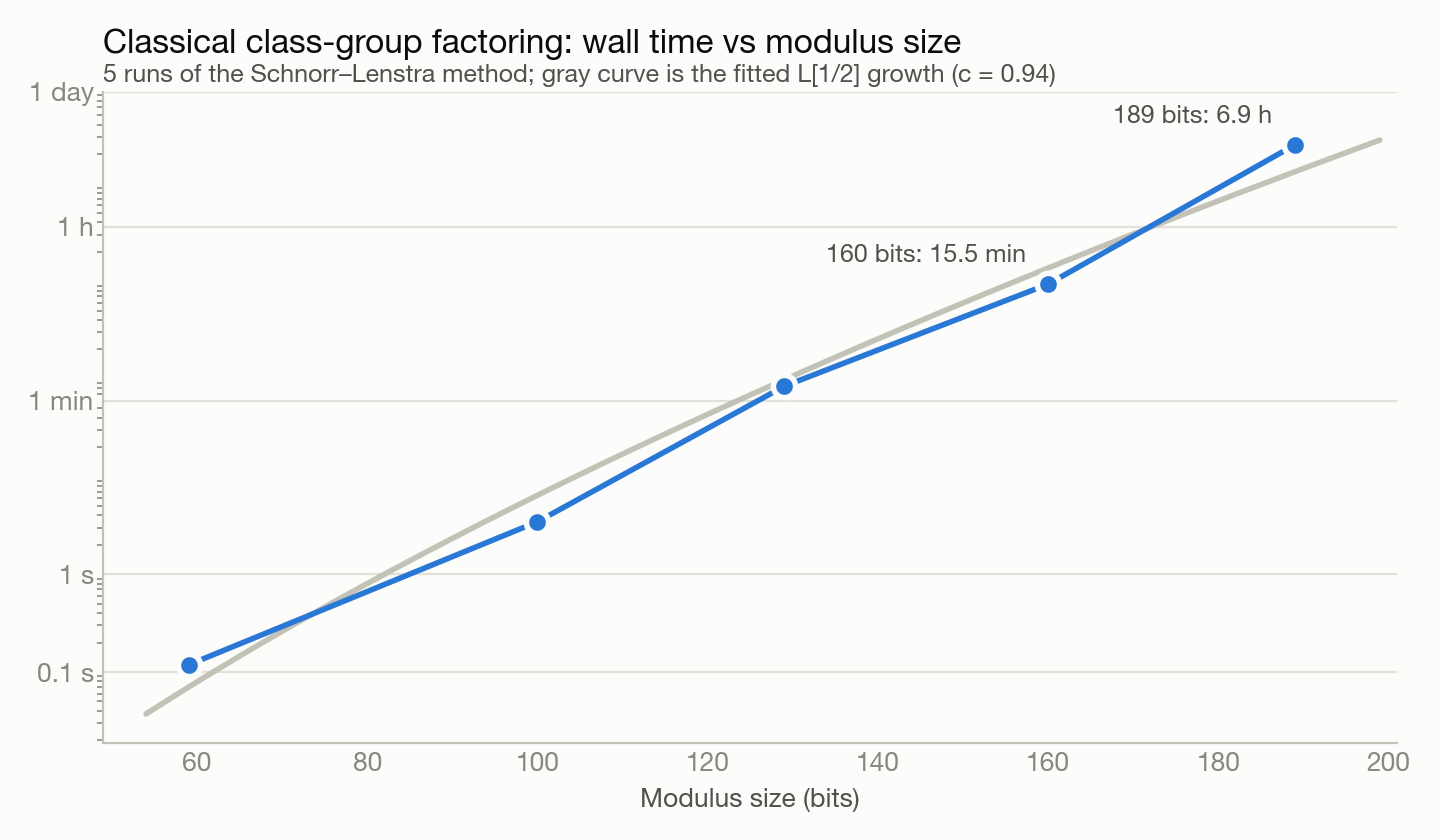
\includegraphics[width=0.8\textwidth]{fig1_scaling.png}
\caption{Wall time of the classical method of Section~\ref{sec:classical} against modulus size, log scale, with the fitted $L[1/2]$ curve in gray ($c=0.94$).}
\label{fig:scaling}
\end{figure}

\subsection{Simulating the quantum sampler}
A uniform point of $L^*/\Z^d$ is a uniformly random character of $\Cl(D)$ evaluated on the generators. Given the cyclic structure of $\Cl(D)$ and the discrete logarithms of the prime forms from PARI's \texttt{bnfinit}, the simulator draws characters, adds noise of magnitude $2^{-\eta}$, rounds to $D'$ bits and feeds the post-processing, exactly as Eker\aa's simulator \cite{ekera_regevnum} uses the factorization to simulate integer Regev. One sign convention between our forms and PARI's ideals was fixed by verifying a known relation by composition. Table~\ref{tab:sim}: in every successful run all $d$ recovered vectors were relations, the recovered lattice had index one in $L$, and the extraction factored $N$. At 99 bits the post-processing tolerated noise to $2^{-12}$ at 48-bit precision and failed at $2^{-9}$. The simulated circuit used $8$ sequential squarings per run on $50$-bit forms against $13$ for integer Regev at the same $d$, as \eqref{eq:total} predicts with the slack $c=3$ used at this size.

\begin{table}[t]
\caption{Simulated Regev runs over $\Cl(-N)$: $d$ generators, $m=d+4$ runs, $B$ exponent bits per generator, $D'$ output bits, noise of magnitude $2^{-\eta}$ added to each sample.}
\label{tab:sim}
\centering
\begin{tabular}{rrrrrrl}
\toprule
bits & $d$ & runs & $B$ & $D'$ & noise & result \\
\midrule
59 & 8 & 12 & 7 & 44 & $2^{-22}$ & index 1, factored, 0.1 s\\
99 & 10 & 14 & 8 & 48 & $2^{-24}$ & index 1, factored, 2.7 s\\
99 & 10 & 14 & 8 & 48 & $2^{-12}$ & index 1, factored\\
99 & 10 & 14 & 8 & 48 & $2^{-9}$ & no relations recovered\\
\bottomrule
\end{tabular}
\end{table}

\subsection{Reproducibility}\label{sec:repro}
All code, the per-experiment results, and the LaTeX source are provided as anonymized supplementary material and will be released publicly with the final version. A single command, \texttt{./reproduce.sh}, reruns every experiment in this paper from fixed seeds, regenerates Tables~\ref{tab:classical}--\ref{tab:cost} and both figures from the results, and builds this PDF; the two slowest classical runs are shipped as recorded results and rerun with \texttt{--full}. Requirements are Python with \texttt{sympy} and \texttt{matplotlib}, PARI/GP, and a TeX distribution. Lemma~\ref{lem:amb} and the group-theoretic part of Theorem~\ref{thm:red} are also machine-checked in Lean~4 with Mathlib, included in the supplementary material. The formalization proves, by integer arithmetic on $\mathrm{SL}_2(\mathbb{Z})$-substitutions, that properly equivalent reduced forms are equal and that a reduced form equivalent to its opposite $(a,-b,c)$ is ambiguous. Since Mathlib has no composition of forms, the class group is an abstract finite abelian group whose classes have distinct reduced representatives, with the principal form as identity and the opposite form as inverse; these are its defining properties, not theorems about it. GRH, used only for near-uniform sampling, is not modelled.

\section{Cost of the Group Operation}\label{sec:cost}
\subsection{Squaring a form}
For reduced $f=(a,b,c)$ with $\gcd(a,b)=1$, let $C\equiv-c\,b^{-1}\pmod a$. Then
\begin{equation}\label{eq:sq}
f^2\sim\tfrac1a f(ax+Cy,\,y)=\big(a^2,\;b+2aC,\;(c+bC+aC^2)/a\big),
\end{equation}
with $a^2\approx N$ to be reduced. A partial Euclid on $(a,C)$ with cofactors $s_j$, $r_j\equiv s_jC\pmod a$, stopped at $|r|\le|D|^{1/4}$, gives unimodular $U$ with $(a,C)U=(d,v)$; substituting into \eqref{eq:sq} with integral $e_1=(bd+cs_0)/a$, $e=(bv+cs_1)/a$ yields the nearly reduced form $(d^2+s_0e_1,\;2dv+s_1e_1+s_0e,\;v^2+s_1e)$. This is NUDUPL \cite{jacobson2002} rederived; its products are on quarter-size numbers except four of size $n/2\times n/4$. Our implementation matched composition followed by reduction on all twelve instrumented 4096-bit squarings, with $1.8$ final reduction steps on average. Instrumented on twelve random 4096-bit forms, in units of $M=(n')^2$ bit-products, $n'=2048$: $7.4M$ of multiplication and division, a full extended GCD of width $n'$ (area $1.0M$), a partial Euclid of width $n'$ over $n'/2$ bits (area $0.5M$), and the reduction of $cu$ modulo $a$, an $n'\times n'$ division (area $1.0M$). Under the convention of Section~\ref{sec:rev} the products and exact divisions cost twice their bit-area and the reduction three times its quotient-by-divisor area, which converts this arithmetic to $2\times7.4+3\times1.0=17.8\,(n')^2$ Toffolis per squaring, the third row of Table~\ref{tab:cost}.

\subsection{Why the inverse is intrinsic}
Equation \eqref{eq:sq} says squaring \emph{is} the inverse: the square is the lattice $\{(x,y):x\equiv Cy\ (\mathrm{mod}\ a)\}$ under the norm form $f$, and $C$ is $-cb^{-1}$. Composition of coprime-norm forms is the isomorphism $\Z/a\times\Z/a'\to\Z/aa'$, an inverse by definition. The redundant generating set $\{(a,0),(0,a),(c,-b)\}$ of the same lattice avoids writing $C$, but reducing it performs the full Euclid on $(a,b)$ in the second coordinate before any shortening. Representatives with $b\equiv\pm1\pmod a$ exist only when $a\mid D-1$. Since $a$ is quantum data, Fermat inversion (needs $\varphi(a)$) and Montgomery precomputation (needs a classical modulus) are unavailable.

\subsection{Reversible circuits}\label{sec:rev}
One convention for both routes: controlled add or subtract of quantum registers of width $w$ costs $2w$ Toffolis, controlled swap $w$, comparison $w$, controlled classical-constant add $w$, $n\times m$ product $2nm$, shifts and CNOTs free. Under it, an integer Regev step at $n=4096$ (product, Montgomery reduction by the classical $N$, multiplication by the subset product, sized for its worst case of $517$ bits, and its reduction) costs $17.0\,(n')^2$.

\paragraph{Modular inverse} Bernstein--Yang divsteps \cite{bernstein2019} with the proven count $K=\lceil(49n'+57)/17\rceil$ give a branch-free loop. We invert $a$ modulo the always-odd $b$, tracking cofactors $(p,q)$ modulo $b$ with $f\equiv pa$, $g\equiv qa$ and a modular halving per step, so no $2^{-K}$ correction arises; $u=(1-va)/b$ converts to $b^{-1}\bmod a$ with one product and one exact division. A divstep is two controlled swaps, two controlled adds with the sign folded into a carry-in, and one modular halving: $8n'+O(\log n')$ Toffolis and two history qubits. At $n'=2048$, $K=5907$, forward cost $23.1\,(n')^2$, correct on every test; uncomputing the $11{,}814$ history qubits doubles it to $46.2\,(n')^2$.

\paragraph{Partial Euclid} A full-width restoring division, then division steps with a six-bit quotient budget, integer cofactors, a done flag at $|r|\le|D|^{1/4}$, and a fixed budget of $0.44n'$ steps. The output was verified as a basis of determinant $a$ in every test: forward $16.4\,(n')^2$, clean $32.8\,(n')^2$. The step budget is not a worst-case bound, and the shortfall cannot be made negligible by enlarging it. A quotient $q$ above the six-bit cap costs about $q/63$ steps, and by the Gauss--Kuzmin law a quotient exceeds $x$ with probability $\log_2(1+1/x)\approx1.44/x$; over the roughly $650$ quotients of one call, overrunning the budget by $E$ steps has probability about $15/E$, of order $5\%$ at the $0.44n'$ budget. The tail decays only like the inverse of the budget, and a wider quotient cap, at a higher cost per step, thins it without changing its shape. A branch of the superposition that exhausts the budget holds a correct but unreduced form, so it no longer interferes with the branches of its class, and the error per run is not below the $2^{-\eta}$ the post-processing needs. A correct circuit must handle large quotients coherently, for example by aligning the leading bits of the operands before each step, which bounds the step count in the worst case at the price of a shift per step. The partial-Euclid cost above is therefore a lower bound for a correct circuit, and every such correction adds class-group cost only.

\paragraph{Qubits} Both accumulators are $n$ bits. The class-group exponent register saves about $2000$ qubits, the Euclid histories cost about $21{,}000$ if kept, and both routes share the cost of retaining or pebbling the non-invertible squaring \cite{ragavan2024}. Qubits do not change the verdict.

\subsection{Comparison}
Table~\ref{tab:cost} and Fig.~\ref{fig:hero} assemble the costs; the small-form composition at $15.8\,(n')^2$, sized like the integer step for the worst-case subset product, and the $1.5\times$ arithmetic uncompute overhead are the only modelled entries besides the integer step. In the clean column the overhead is $1.5\times$ on arithmetic and $2\times$ on Euclidean histories for both routes: the small-form row is $1.5\times8.2+2\times7.7=27.6$, and the integer step, all arithmetic, becomes $25.5$. Per step the class group costs $4.3\times$ (garbage kept) or $5.2\times$ (clean) the integers. Equation \eqref{eq:total} gives $2720$ against $4896$ total squarings at $d=64$, a factor $0.56$, so the totals are $2.4\times$ and $2.9\times$. Since the partial-Euclid entry is a lower bound for a correct circuit (Section~\ref{sec:rev}), these ratios are lower bounds as well; a design with a guaranteed step count would only raise them. In units of one $n'$-bit product, $2(n')^2$ Toffolis, the modular inverse alone costs $11.6$ products and the inverse with the partial Euclid $19.8$ (garbage kept) or $39.5$ (clean). Break-even would require all Euclidean work, including the small-form composition's, to fit in the budget that \eqref{eq:total} leaves after the arithmetic ($17.8+8.2=26.0$ kept, $26.7+12.2=38.9$ clean): $17.0/0.556-26.0\approx4.6$ units, or $2.3$ products, with garbage kept, and $25.5/0.556-38.9\approx7.0$ units, or $3.5$ products, clean. The published inverse-to-multiplier ratios $4.2$ \cite{roetteler2017} and $13.5$ \cite{luo2026b} are measured against those papers' own multipliers rather than a $2n^2$ product, so they do not transfer to this comparison.

\begin{table}[t]
\caption{Toffoli cost of one sequential squaring step at $n=4096$, in units of $(n')^2$ with $n'=2048$, under the convention of Section~\ref{sec:rev}.}
\label{tab:cost}
\centering
\begin{tabular}{lrr}
\toprule
component & garbage kept & clean \\
\midrule
modular inverse (measured) & 23.1 & 46.2\\
partial Euclid (measured) & 16.4 & 32.8\\
NUDUPL products, divisions (measured) & 17.8 & 26.7\\
small-form composition (modelled) & 15.8 & 27.6\\
\midrule
class-group step & 73 & 133\\
integer Regev step (modelled) & 17.0 & 25.5\\
total ratio after $\times0.56$ & $2.4\times$ & $2.9\times$\\
\bottomrule
\end{tabular}
\end{table}

\section{Discussion}\label{sec:disc}
\subsection{Group size and the modulus}\label{sec:floor}\label{sec:modulus}
Two heuristic remarks suggest why the halving and the inverse arrive together; neither is a theorem. First, if $p$, about $n/2$ bits, is to be read off the order of $G$ or of a subgroup, an integer of at most $\log_2|G|$ bits, then $|G|\gtrsim2^{n/2}$, and by \eqref{eq:total} the total number of sequential squarings is at least about $n/2$. The groups $(\Z/N\Z)^*$, elliptic curves over $\Z/N\Z$ and algebraic tori have size about $N$ and pay $n$; $\Cl(-N)$ has size about $\sqrt N$ and pays $n/2$. Second, inverse-free arithmetic, by projective coordinates or Montgomery reduction, needs a known classical modulus. The classical moduli available are $N$ and functions of it, and a classical number of size about $\sqrt N$ that constrained $p$ modulo itself would essentially determine $p$. Orders of conductor $f$ in a class-number-one field have inverse-free arithmetic modulo $f$, but their Picard groups have size about $f$, so at $f=N$ the group size returns to about $N$. We therefore expect a group of size about $\sqrt N$ that exposes $p$ to pay for an inverse modulo quantum data, as $\Cl(-N)$ does.

\subsection{What would change the verdict}
Only a near-elimination of the Euclidean work. Break-even leaves $4.6$ units for all of it with garbage kept and $7.0$ clean, against $47.2$ and $94.5$ for the inverse, the partial Euclid and the small-form composition's Euclid together, a factor of $10$ to $14$. A cheaper divstep cannot supply this: even a free modular inverse leaves the route at $1.6\times$ ($1.9\times$ clean), and with every Euclidean step free the class group would win by only $15\%$. The candidates are a sub-quadratic reversible GCD, since half-GCD recursion gives $O(M(n)\log n)$ classically, but no reversible version with known constants at 2048 bits exists, and the recursion's workspace is the obstacle; or a different model of $\Cl(-N)$ with inverse-free arithmetic, which Section~\ref{sec:modulus} argues would require a classical modulus of size $\sqrt N$, which would itself determine $p$. The real quadratic variant through the infrastructure of $\Q(\sqrt N)$ changes none of this; its giant step is the same composition with a distance attached, and its advantage, a Shor-shaped single run, is exactly what Regev's structure gives up for shallower circuits.

\subsection{Limitations}
Three entries of Table~\ref{tab:cost} are modelled: the integer step, the small-form composition, and the $1.5\times$ uncompute overhead, applied alike to both routes' arithmetic. The reversible designs were executed as classical simulations of reversible primitives with a cost ledger, not synthesized in a circuit framework, so shared constants such as adder uncomputation are approximate on both sides. The partial-Euclid step budget was set at $1.15\times$ the observed maximum plus $8$; as Section~\ref{sec:rev} explains, no budget for six-bit quotients makes the failure negligible, so its cost is a lower bound. The short-basis assumption for class-group relation lattices rests on the Gaussian heuristic and the index-one recoveries. Forms with $\gcd(a,b)>1$ need no circuit: a common divisor of $a$ and $b$ divides $b^2-4ac=-N$, so it is $p$ or $q$, and a branch that meets one has already factored $N$; for a near-uniform class this has probability heuristically about $2^{-n/2}$, and none of our 4096-bit samples met it. None of this affects the sign, and the corrections a correct circuit needs only raise the class-group cost: the measured Euclid components alone are $2.3\times$ the integer step before any arithmetic is counted.

\section{Conclusion}
Regev's algorithm over the class group of $\Q(\sqrt{-N})$ is, for $N\equiv3\pmod4$, a correct polynomial-time factoring algorithm with half the sequential group operations of the integer version, extracting the factorization deterministically from the $2$-torsion. It loses by at least $2.4\times$ ($2.9\times$ fully uncomputed) at 4096 bits because form squaring contains a modular inverse with respect to quantum data costing about a dozen multiplications even branch-free. Reopening the question would take a tenfold reduction of all Euclidean work, which no improvement of the divstep provides; a sub-quadratic reversible GCD with small constants at 2048 bits is the candidate we see. Absent those, class groups do not help Regev-style factoring, and this paper is meant as the reference answer to why.

\subsubsection*{Disclosure of AI Assistance.}
This work was carried out in an interactive session with a large language model (Claude, Anthropic), which drafted the code, the cost analysis, and the manuscript text under the authors' direction. The authors take full responsibility for the content. Every numerical result in the paper is produced by the public code from fixed seeds and was regenerated by \texttt{reproduce.sh} before submission; the proofs in Section~\ref{sec:prelim} and the arguments in Section~\ref{sec:disc} were checked by the authors; every reference was verified against its source.

\bibliographystyle{splncs04}
\bibliography{refs}
\end{document}
